%Matteo Kumar - Leonard Schatt
% Fortgeschrittenes Physikalisches Praktikum

% Teilauswertung SE

\section{Spektrale Empfindlichkeit}
\subsection{Lock-in-Verstärker}
Um den Photostrom $I_{Ph}$ zu berechnen, muss zunächst die am Lock-in-Verstärker abgelesene Spannung in die tatsächlich anliegende Spannung umgerechnet werden. Der Verstärker hat als Output einen Wert zwischen $0$V und $10$V. Berücksichtigt man noch die Sensitivity des Verstärkers erhält man für die anliegende Spannung $U_{rms}$: \\

\begin{equation}
U_{rms} = \frac{U_{angezeigt}}{10V} \cdot Sensitivity
\end{equation}

Nun muss noch berücksichtigt werden, dass der Lock-in-Verstärker das Messsignal, das durch den Chopper (annähernd) reckteckförmig moduliert wurde, mit dem sinusförmigen Referenzsignal des Choppers faltet, bevor die Faltung durch einen Tiefpass geleitet wird. Ein Rechtecksignal kann geschrieben werden als:\\

\begin{equation}
f_{Rechteck} = \frac{4U_{Rechteck}}{\pi} \sum_{k=1}^\infty \frac{sin((2k-1)\omega t)}{2k-1}  ,
\end{equation}

wobei $U_{Rechteck}$ die Amplitude des Signals bezeichnet.
Faltet man dieses nun mit einem Signal der Frequenz $\omega$, so trägt nach durchlaufen des Tiefpasses nur der Anteil am Rechtecksignal mit ebenfalls $\omega$ bei, also der Term für $k = 1$. Die gemessene Spannung ergibt sich also zu: \\

\begin{align}
U_{ein} &= \frac{4U_{Rechteck}}{\pi} sin(\omega t) \nonumber \\ 
\implies U_{rms} &= \frac{1}{\sqrt{2}} \frac{4U_{Rechteck}}{\pi}
\end{align}

Stellt man nun nach der Amplitude der Spannung $U_{Rechteck}$ um, so erhält man:

\begin{align}
U_{Rechteck} &= \frac{\pi \sqrt{2}}{4} U_{rms} \\
\implies U_{Rechteck} &= \frac{\pi \sqrt{2}}{4} \cdot Sensitivity \cdot \frac{U_{angezeigt}}{10V}
\end{align}

Um den Photostrom $I_{Ph}$ zu erhalten, muss jetzt nur noch die tatsächliche Spannung mithilfe des Faktors des U/I-Verstärkers umgerechnet werden:\\

\begin{align}
I_{Ph} &= \frac{U_{Rechteck}}{1 \frac{kV}{A}} \nonumber \\
 &= \frac{\pi \sqrt{2}}{4} \cdot Sensitivity \cdot \frac{U_{angezeigt}}{10000 \frac{V^2}{A}}
\label{eq:IPh}
\end{align}


\subsection{Spektrale Empfindlichkeit SR und Externe Quanteneffizienz EQE}

Die Spekrtale Empfindlichkeit $SR$ berechnet sich nach:
\begin{equation}
SR = \frac{I_{Ph}}{P_\lambda},
\end{equation}

mit Photostrom $I_{Ph}$ aus Gl. \ref{eq:IPh}. Dabei muss noch berücksichtigt werden, dass für alle Messwerte noch der Photostrom aus der
Untergrundsmessung abgezogen wird. \\
Die in die Zelle einfallende Leistung $P_{\lambda}$ muss erst noch aus der in das Powermeter einfallende Leistung berechnet werden. Es gilt:
\begin{align}
P_{PM} &= P_{ges} R \nonumber \\
P_{\lambda} &= P_{ges} T \nonumber \\
\implies P_{\lambda} &= P_{PM} \frac{T}{R},
\end{align}

mit Reflektionskoeffizient des Strahlteilers $R$, Transmissionskoeffizient $T$ und gesamter Lichtleistung vor Auftreffen auf den Teiler $P_{ges}$.
Für die Werte von $\frac{T}{R}$ wurden die Inversen von Abschätzungen der Werte $\frac{R}{T}$ aus Anhang $A.2$ des Versuchsskriptes benutzt.

Aus den Werten für $SR$ lassen sich nun auch die für die Externe Quanteneffizienz $EQE$ berechnen:
\begin{align}
EQE &= \frac{hc}{e} \frac{SR}{\lambda}
\label{eq:eqe}
\end{align}

Die berechneten Werte finden sich in Tab. ref. wieder. TABELLEN!!
\\

Die Lage der Bandkanten sind für Silizium $1,1242$eV (Quelle: https://www.pveducation.org/pvcdrom/materials/general-properties-of-silicon, 9.9.21) und für CIS $1,02$eV. (Quelle:https://www.pveducation.org/pvcdrom/materials/cuinse2, 9.9.21). Die Lage dieser im Wellenängenraum berechnet sich nach. \\

\begin{align}
\lambda_{Bandkante} &= \frac{hc}{E_{Bandkante}}
\end{align}

Daraus folgt: \\

\begin{equation}
\lambda_{Si} = 1102,866 nm, \qquad \lambda_{CIS} = 1215,531 nm
\label{eq:bandkante}
\end{equation}

In den folgenden Abbildungen \ref{bild:SiSRMess} - \ref{bild:CISEQE} wurden die spektrale Empfindlichkeit und die externe Quanteneffizienz gegen die Wellenlänge aufgetregen.
Dabei wurden auch die jeweiligen Bandkanten aus Gl. \ref{eq:bandkante} eingezeichnet.
Zunächst fällt auf, das die Werte für die Siliziumzellen in beiden Graphen ungefähr um den Faktor zehn größer sind als die der 
CIS-Zellen. Vor allem bei der $EQE$ ist aber klar, dass dies nicht realistisch ist, da für diese $0 < EQE < 1$ gelten muss.
In Annahme, dass die (einfache) Umrechnung von $SR$ in $EQE$ korrekt ist (dies legt auch der sinnvolle Verlauf des Graphen für 
das CIS-Modul nahe), und dass beim Übertragen der Rechnung keine Fehler gemacht wurden, sind Mess- oder Methodikfehler als Fehlerquellen
wahrscheinlich. Als Ergänzung sind in Abb. \ref{bild:allSRgest} und \ref{bild:allEQEgest} die um den Faktor 10 gestauchten Graphen gezeigt.
 Bei den Siliziummodulen ist zu erkennen, dass trotz 
Überschreitung der Bandkante nicht vernachlässigbare Leistungen im Powermeter gemessen wurden. Dies ist auch nicht alleine durch die 
Driftleistung des Powermeters zu erklären, da diese im Nanowatt-Bereich liegen. 
Die Bandkante des CIS-Moduls liegt bei einer höheren Wellenlänge als der Messpunkt der größten Wellenlänge, deshalb kann nicht mit 
Sicherheit gesagt werden, ob das Problem des Überschreitens der Bandkante hier auch auftreten würde. Dennoch lässt sich an Abb. 
REFERENZ gut erkennen, dass die Lage der Bandkante annäherungsweise mit dem Nulldurchgang des Graphen der spektralen Empfindlichkeit
übereinstimmt. Als Erklärung, dass hinter der Bandkante noch Messwerte vorliegen, können Messfehler dienen. Allerdings ist die 
Überschreitung nicht sehr groß, daher kann auch eine Abweichung der realen Solarzelle vom Bändermodell die Ursache sein. \\

\begin{figure}[h]
    \centering
    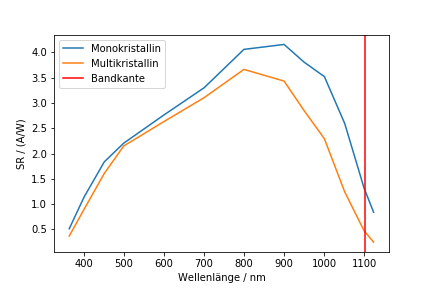
\includegraphics[scale=0.75]{Bilder/32_Si_SR.png}
    \caption{Verlauf der gemessenen Werte von $SR$ der Siliziumzellen aufgetragen gegen die Wellenläge}
    \label{bild:SiSRMess}
\end{figure}

\begin{figure}[h]
    \centering
    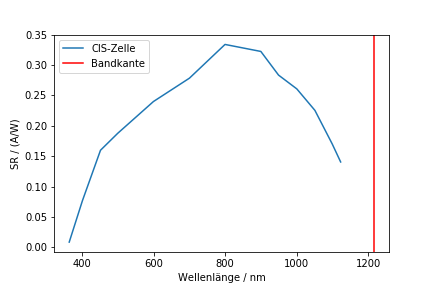
\includegraphics[scale=0.75]{Bilder/32_CIS_SR.png}
    \caption{Verlauf der gemessenen Werte von $SR$ der CIS-Zelle aufgetragen gegen die Wellenläge}
    \label{bild:CISSR}
\end{figure}



\begin{figure}[h]
    \centering
    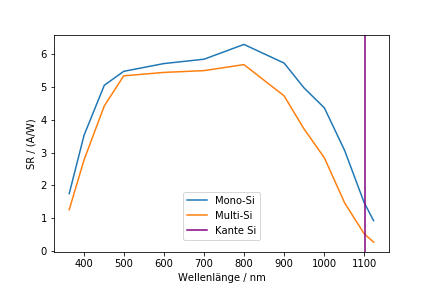
\includegraphics[scale=0.75]{Bilder/32_Si_EQE.png}
    \caption{Verlauf der gemessenen Werte von $EQE$ der Siliziumzellen aufgetragen gegen die Wellenläge}
    \label{bild:SiEQE}
\end{figure}

\begin{figure}[h]
    \centering
    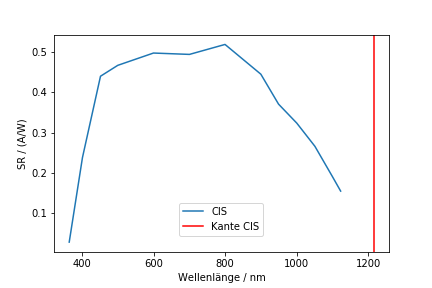
\includegraphics[scale=0.75]{Bilder/32_CIS_EQE.png}
    \caption{Verlauf der gemessenen Werte von $EQE$ der CIS-Zelle aufgetragen gegen die Wellenläge}
    \label{bild:CISEQE}
\end{figure}

\begin{figure}[h]
    \centering
    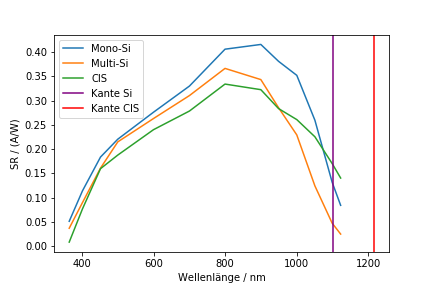
\includegraphics[scale=0.75]{Bilder/32_all_SR_gest.png}
    \caption{Verlauf der um den Faktor zehn gestauchten Werte von $SR$ der Siliziumzellen aufgetragen gegen die Wellenläge, zusätzlich
    zu dem Verlauf der CIS-Zelle}
    \label{bild:allSRgest}
\end{figure}

\begin{figure}[h]
    \centering
    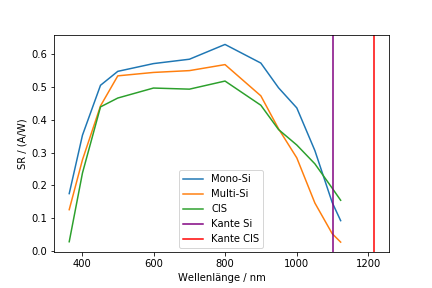
\includegraphics[scale=0.75]{Bilder/32_all_EQE_gest.png}
    \caption{Verlauf der gemessenen Werte von $EQE$ aller Zellen aufgetragen gegen die Wellenläge; Werte für Si-Zellen um Faktor
    zehn gestaucht}
    \label{bild:allEQEgest}
\end{figure}

Als Anhaltspunkt zum Vergleich sollen die Abb. \ref{bild:ThSR} und \ref{bild:ThEQE} dienen, in denen $SR$ und $EQE$ für eine multikristalline Solarzelle 
gegen die Wellenlänge aufgetragen ist. Es ist gut zu erkennen, dass der grobe Verlauf mit den gemessenen Kurven übereinstimmt. Dies
legt nahe, dass es sich beim Fehler bei den Siliziumzellen tatsächlich nur um einen Fehler um einen Faktor ca. 10 handelt. Im 
Vergleichsgraphen werden zwar deutlich höhere Werte für $SR$ und $EQE$ erreicht, es ist aber anzunehmen, dass der Idealitätsfaktor $n$ 
der dort in präzisen Labormessungen verwendeten Zellen deutlich besser war und dass infolgedessen die Ausbeute höher war.
Aber auch in diesen Messungen ist deutlich zu sehen, dass die Bandkante bei $\lambda = 1102,866 nm$ deutlich überschritten wird. Somit
kann das Überschreiten in unserer Messung wahrscheinlich auf die Abweichungen der realen Zelle im Bändermodell zurückgeführt werden.

\begin{figure}[h]
    \centering
    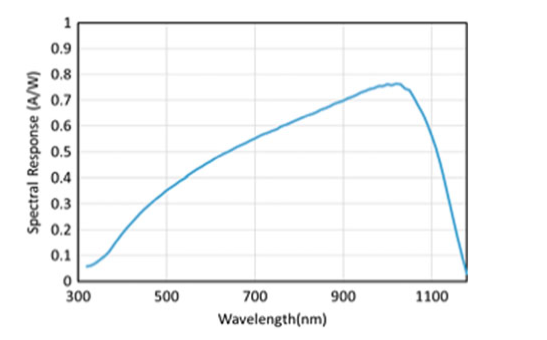
\includegraphics[scale=0.75]{Bilder/Theorie_SR.png}
    \caption{Vergleichsdaten für den Verlauf von $SR$ einer multikristallinen Siliziumzelle}
    \label{bild:ThSR}
\end{figure}

\begin{figure}[h]
    \centering
    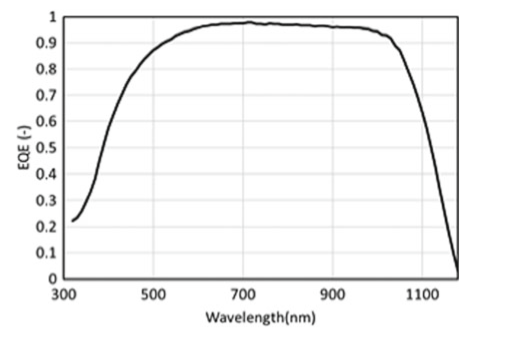
\includegraphics[scale=0.75]{Bilder/Theorie_EQE.png}
    \caption{Vergleichsdaten für den Verlauf von $EQE$ einer multikristallinen Siliziumzelle}
    \label{bild:ThEQE}
\end{figure}

Quelle: beide: Shah, S.68



\subsection{Ideale Externe Quanteneffizienz}

Nimmt man nun eine ideale externe Quanteneffizienz von $1$ an, folgt aus Gl. \ref{eq:eqe}:
\begin{align}
SR &= \frac{e}{hc}\lambda
\end{align}

Der Graph der spektralen Empfindlichkeit ist somit zunächst eine Gerade mit Steigung $\frac{e}{hc}$, bis diese Gerade auf die
Vertikale der bandkante trifft. Da nach Überschreitung der Bandkante kein Stromfluss mehr möglich ist (höhere Wellenlänge 
$\leftrightarrow$ niedrigere Energie), fällt die Gerade dort abrupt ab. Der Verlauf ist in Abb. \ref{bild:idealEQE} zu sehen.
Hierbei ist der Verlauf beider Modularten erst die rote Ursprungsgerade, die dann im Fall der Siliziumzellen mit der violetten
Vertikalen, im Fall des CIS-Moduls mit der roten Vertikalen abfallen.
Hier wird 
nochmals klar, dass die Werte der Siliziumzellen für $SR$ nicht stimmen können, da sie besser als der Idealverlauf wären.
Betrachtet man die Graphen der Messwerte wird klar, dass die verwendeten Zellen fern von einem Ideal sind. Dieser Umstand soll in der
nächsten Teilaufgabe weiter vertieft werden, wenn der Idealitätsfaktor bestimmt wird.

\begin{figure}[h]
    \centering
    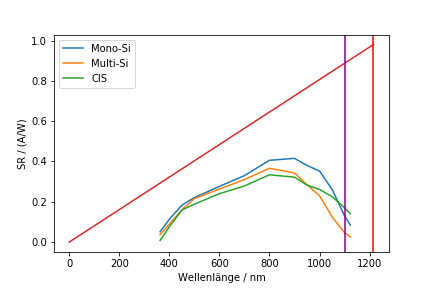
\includegraphics[scale=0.75]{Bilder/32_ideal_EQE.png}
    \caption{Verlauf von $SR$ bei einer idealen $EQE = 1$; der Graph für die Si-Zellen fällt mit der violetten Vertikalen ab, der für
    das CIS-Modul mit der roten. Zum Vergleich die Messwerte für $SR$ (Si-Zellen um Faktor 10 gestaucht)}
    \label{bild:idealEQE}
\end{figure}

